\subsection{Docker}
\label{sec:docker}
Docker plays a pivotal role in this project, serving as an integral tool. 
It offers a clean and efficient means of running instances that essentially 
need to be isolated once they have completed their execution. 
This allows for the encapsulation of the machines or infrastructure used for the \ac{CTF} within Docker images, 
which can then be shared with other systems. When these images are executed on those systems, the expectation is to achieve consistent outcomes.

\subsubsection{What is Docker?}
Docker\cite{docker-docs} is an open platform used for developing, shipping, and running applications. 
It utilizes containers, which are isolated environments for running specific applications. 
Containers are lightweight and encapsulate everything needed for an application to run, 
eliminating the need for the host machine to have specific dependencies installed

\begin{figure}[h]
    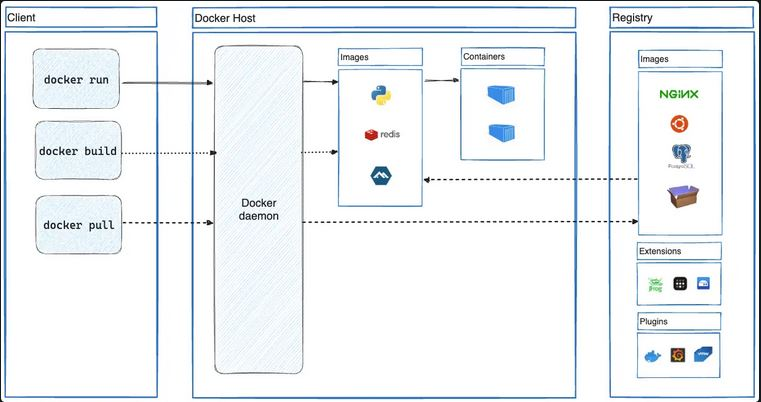
\includegraphics[scale=.7]{images/Docker-architecture.jpg}
    \caption{Docker architecture\cite{docker-docs}}
    \label{fig:docker_architecture}
\end{figure}

The architecture of docker is client-server. 
As seen in figure \ref{fig:docker_architecture} Docker consist of mostly 3 parts; client, daemon (host) and the registry.
The client is the \ac{CLI} which is used as an intermediary to communicate with the daemon. 
The daemon handles everything related to the containers, like building, running, and distributing them.
When images are not stored locally on a users machine or server, they are fetched from the registry.
The registry is a place where images are stored and can be fetched from. There is a many 
authorized registries, but the most common one is Docker Hub.\cite{dockerhub}\\
\paragraph{\textbf{What is a container?}}
A container\cite{docker-concepts} is an isolated process. 
That means that it's a process that runs on a host machine, but it's isolated from the host machine.
Containers can also be described as a lightweight \ac{VM}. Containers are also isolated from each other, but they share the same kernel.
Therefore containers act like components in a bigger project, meaning if a user wants to run a web-application, he or she might need a frontend, database, \ac{API}, etc.
All these things can be isolated from each other, but still have the ability to communicate with each other.
\paragraph{\textbf{What is an image?}}
A container is only as powerful as it's configuration, and for configuring a containers,
Docker uses images\cite{docker-concepts}.\\
Images are the configuration of the container.
They are used to create containers. Images are read-only, meaning that they can not be changed once build.
To change an image, one would to rebuild it from scratch.
For Docker to work, the parts has to work together in harmony. The client sends a request to the daemon, which then executes the request.
If the image isn't stored locally it fetches it or builds it. Once an image is locally present and complete the daemon  
will create a container from the image.
When using the Docker CLI things can quickly become complicated, but with the help of \javaf{docker-compose}, things can be simplified.
\subsubsection{\javaf{docker-compose}}
Docker compose is a tool for running multi-container applications. With the help of \ac{YAML}\cite{YAML}
and a configuration file name \javaf{docker-compose.yml}, it is possible to define services to run.
The docker compose\cite{docker-compose} application model consist of the main 3:
\begin{itemize}
    \item \javaf{Services} is a definition of a containerized application or components of an application. For the Docker compose file,
    this is where the definition of the services that going to be spawn that make the \javaf{docker-compose} file a multiple container application.
    \item \javaf{Networks} is a definition of a virtual network that containers can connect to, in order to communicate with each other.
    If no network is specified, the containers will be connected to the default network. In Docker compose it is possible for 
    containers via Docker internal \ac{DNS} to communicate with each other. 
    This means that even though that IP's might change, the containers can find and communicate with another container through it \ac{DNS} record.
    \item \javaf{Volumes} are a way to persist data generated by containers or share data between containers and the host system. 
\end{itemize}
When combining these three elements, it is possible create a multi-container application. The \javaf{docker-compose} file is a 
\ac{YAML} file that defines the services, networks, and volumes that is going to spawned. Once a developer
has defined everything needed in the \javaf{docker-compose} file, the multi-container application 
can be spawned with a single command, \javaf{docker-compose up}. As there can be many ways to define a \javaf{docker-compose} file, 
we'll wait until section \ref{sec:technical_implementation} to see the \javaf{docker-compose} file that is used in this project.
\newpage